\documentclass[11pt]{article}
\usepackage{tikz}
\usepackage{pifont}
\usepackage{amsmath}
\usepackage{marvosym}
\usepackage{verbatim}
\usepackage{listings}
\usepackage[utf8]{inputenc}
\usepackage{subfig}
\usepackage[switch,columnwise]{lineno}
\usepackage{amssymb}
\usepackage{enumitem}
\usepackage[nottoc,numbib]{tocbibind}
   
\usepackage{hyperref}
\hypersetup{
bookmarks=false,         % show bookmarks bar?
unicode=true,          % non-Latin characters in Acrobat's bookmarks
pdftoolbar=true,        % show Acrobat's toolbar?
pdfmenubar=true,        % show Acrobat's menu?
pdffitwindow=true,     % window fit to page when opened
pdfstartview={FitH},    % fits the width of the page to the window
pdftitle={Node allocators},    % title
pdfauthor={Marcelo Zimbres},     % author
pdfsubject={C++ allocators},   % subject of the document
pdfcreator={Marcelo Zimbres},   % creator of the document
pdfproducer={Marcelo Zimbres}, % producer of the document
pdfkeywords={allocators} {C++}, % list of keywords
pdfnewwindow=true,      % links in new window
colorlinks=true,        % false: boxed links; true: colored links
linkcolor=red,          % color of internal links
citecolor=red,        % color of links to bibliography
filecolor=red,      % color of file links
linktocpage=true,
urlcolor=blue           % color of external links
}

\lstset{
  language=C++,                 % the language of the code
  backgroundcolor=\color{white},   % choose the background color; you must add \usepackage{color} or \usepackage{xcolor}
  basicstyle=\footnotesize,        % the size of the fonts that are used for the code
  breakatwhitespace=false,         % sets if automatic breaks should only happen at whitespace
  breaklines=true,                 % sets automatic line breaking
  keywordstyle=\color{blue},       % keyword style
  captionpos=b,                    % sets the caption-position to bottom
  commentstyle=\color{blue},       % comment style
  deletekeywords={},            % if you want to delete keywords from the given language
  escapeinside={\%*}{*)},          % if you want to add LaTeX within your code
  extendedchars=true,              % lets you use non-ASCII characters; for 8-bits encodings only, does not work with UTF-8
  frame=single,                    % adds a frame around the code
  keepspaces=true,                 % keeps spaces in text, useful for keeping indentation of code (possibly needs columns=flexible)
  morekeywords={using, static_assert},            % if you want to add more keywords to the set
  numbers=left,                    % where to put the line-numbers; possible values are (none, left, right)
  numbersep=10pt,                   % how far the line-numbers are from the code
  numberstyle=\tiny\color{black}, % the style that is used for the line-numbers
  rulecolor=\color{black},         % if not set, the frame-color may be changed on line-breaks within not-black text (e.g. comments (green here))
  showspaces=false,                % show spaces everywhere adding particular underscores; it overrides 'showstringspaces'
  showstringspaces=false,          % underline spaces within strings only
  showtabs=false,                  % show tabs within strings adding particular underscores
  stepnumber=1,                    % the step between two line-numbers. If it's 1, each line will be numbered
  stringstyle=\color{red},     % string literal style
  tabsize=2,                       % sets default tabsize to 2 spaces
  title=\lstname                   % show the filename of files included with \lstinputlisting; also try caption instead of title
}

\colorlet{blah}{brown!60!black} % box color

\begin{document}

\date{}
\title{ \bf Improving allocator interface for node-based containers}
\maketitle
\noindent
%\vspace{-1cm} \\
{\bf Document number}:  1 \\
{\bf Date}:  \today \\
{\bf Project}: Programming Language C++ \\
{\bf Author}: Marcelo Zimbres (\href{mailto:mzimbres@gmail.com}{mzimbres@gmail.com}) 

\vspace{1cm}

\noindent
{\bf Abstract: }This is a non-breaking proposal to the C++ standard that aims
to reduce allocator complexity, support realtime allocation and improve
performance of node-based containers by making a clear distinction between {\it node}
and {\it array} allocation in the \texttt{std::allocator\_traits} interface.
Two new member functions are proposed \texttt{allocate\_node} and
\texttt{deallocate\_node}. We also propose that the container node type should
be exposed to the user. A prototype implementation is provided.

\vfill
%\newpage
%\twocolumn
%\linenumbers
\begin{flushright}
\noindent
{\it Size management adds undue difficulties \\
     and inefficiencies to any allocator design} \\
A. ALEXANDRESCU \\
\medskip
{\it }
\end{flushright}
\medskip

\newpage
\tableofcontents

\newpage
\section{Introduction}
\textsc{The importance} of linked data structures in computer science, like
trees and linked lists, cannot be over-emphasised, yet, in the last couple of
years it has become a common trend in C++ to move away from such data
structures due to their sub-optimal memory access patterns \cite{middleditch,
chandler, meyers}.  In fact, many people today prefer to use the flat
alternatives and pay $O(n)$ insertion time, than $O(1)$ at the cost of memory
fragmentation and unpredictable performance loss.  

We believe in fact, that the ``{\it Don't pay for what you don't use}" premise
is not being met on node-based containers due to the restrictive
array-oriented allocator interface. This proposal tries to fix what the author
believes to be the root of problem: {\it The lack of distinction between array
and node allocation}.  We propose here a complete split between these two
allocation techniques by means of a non-breaking addition to
\texttt{std::allocator\_traits}.

\subsection{Node allocation}
%\medskip
%\noindent
%{\bf How simple is node allocation}.
Node allocation is one of the simplest allocation techniques
we can get, but yet a very powerful one. The simplicity
comes from the fact that allocation and deallocation reduces to pushig and
popping from the linked list of nodes, like shown in the code below.
It is powerful because it is very fast, perform in hard-real-time
and cause minimal memory fragmentation.

\medskip
\begin{lstlisting}
pointer allocate(size_t /*can't handle n*/)
{
  pointer q = avail; // The next free node
  if (avail)
    avail = avail->next;

  return q;
}

void deallocate(pointer p, size_t /*can't handle n*/)
{
  p->next = avail;
  avail = p;
}

\end{lstlisting}

The reasons why this allocation technique is not fully supporte in C++ is
related to the current {\it array} oriented interface of allocators.  The
member function \texttt{allocate(n)} may be called with $n \ne 1$, meaning that
the allocator now has to implement array allocation strategies instead of much
more simple and efficient node allocation.

Before going into more details, let us see with a use case,
how this proposal provides better solution over the current
array oriented interface.

\subsection{Use case}
%\medskip
%\noindent
%{\bf Use case}.
The example below uses the allocation technique from the previous section to
write code that is fast, simple and uses the minimum amount of memory. A linked
lists served with a couple of nodes allocated on the stack
\medskip
\begin{lstlisting}
  using alloc_t = rt::node_allocator<int>;

  using node_type = typename std::list<int, alloc_t>::node_type;

  // Buffer for 100 elements.
  std::array<char, 100 * sizeof (node_type)> buffer = {{}};

  alloc_t alloc(buffer);

  std::list<int, alloc_t> l1(alloc);
  ...
  // Inserts elements. Allocation and deallocation implemented
  // with 6 lines of code. Faster and simpler than any allocator
  // I could find.
  l1 = {27, 1, 60};
  ...
\end{lstlisting}

Some of the features of this code are
\begin{itemize}

\item It uses the container node type, to calculate the minimum amount of
memory to support 100 elements in the list. As a consequence the buffer is
compact, improving cache locality and causing minimal fragmentation.

\item The allocator knows it is doing node allocation and does not make the
node size bigger to store bookkeeping information. {\it You do not pay for
space you do not use}. 

\item Very simple and fast allocator where allocation and deallocation
translates into only a couple of pointers assignments. No array allocation
strategy had to be implemented.
%\item {\it It cannot be written portably in C++}.
\end{itemize}

The reasons why we cannot write this code in current C++ will
be better explained below, but shortly said

\begin{itemize}

\item The allocator {\it has to} provide array allocation since 
\texttt{allocate(n)} may be called with $n \ne 1$, as a result
the allocator gets unnecessarily complicated and the size of the
buffer to support 100 elements is not anymore clear since it depends
on the array allocation strategy/algorithm.

\item The container node type and therefore its size is unknown.

\end{itemize}

\subsection{Exposing the node type}

In current C++, there is no straightforward way of knowing the size of the node
the allocator will serve.  At runtime it is known only when the rebound
allocator instance is constructed, which occurs when the container is
constructed. It is a tricky to use this information. As shown in the example
above the user may want to use it to pre-allocate space for a
certain number of elements.

Another situation where the node type is useful is when implementing node
allocators for unordered containers. Usually, unordered containers rebound
twice and there is no way of knowing which rebound type is used for array and
node allocation. Once the node type is exposed the allocator can be specialized
for the desired type, offering node allocation functions accordingly.

Please, see appendix \ref{saferalloc} for an example of how we can write a safe
allocator interface once the node type is exposed.

%We require that the exposed node type support SCARY 
%initialization \cite{scary}. The following should hold
%\medskip
%\begin{lstlisting}
%using node_type1 = std::set<int, C1, A1>::node_type;
%using node_type2 = std::set<int, C2, A1>::node_type;
%using node_type3 = std::set<int, C1, A2>::node_type;
%
%static_assert(std::is_same<node_type1, node_type2>::value, "");
%static_assert(std::is_same<node_type1, node_type3>::value, "");
%static_assert(std::is_same<node_type2, node_type3>::value, "");
%\end{lstlisting}


\subsection{Further considerations}
The influence of fragmentation on performance is well known on the C++
community and subject of many talks in conferences therefore I am not going to
repeat results here for the sake of readability. The interested reader can
refer to \cite{chandler, meyers} for example.

The split between array and node allocation has been successfully implemented
in the Boost.Container library, but the mechanism is based on C++03 instead of
\texttt{std::allocator\_traits}.

For an allocator that explores the feature proposed here, please see the
project \cite{rtcpp}. For a general talk on allocators and why size management
is a problem \cite{alexandrescu}. For related proposal, please see
\cite{prop1}.  For an alternative approaches to support node allocation, please
see appendix \ref{alternative}.

\section{Motivation and scope}

Given the popularity of the standard allocator, it is important to give reasons
why it should be avoided as a first option for node allocations. I will focus
on the use case shown above, where we want to serve an
\texttt{std::list<int>} with a certain number of nodes.

\subsection{Why avoid the standard allocator}

\begin{enumerate}

\item Nodes go on the heap. For only 100 elements I would preferably
use the stack.

\item The node size is small ($\approx 20$bytes), it is not recommended
allocating them individually on the heap. Fragmentation begins to play a role
if I have many lists (or bigger n).

\item  Each heap allocation is an overhead: all the code inside malloc, plus
system calls and allocation strategies. (I only need 20bytes of space for a
node!). Most importantly, the standard allocator does not
know we are doing node allocations and cannot optimize it.

\item Unknown allocated size. Does it allocate more space to store information
needed by the algorithm? How much memory I am really using?

\end{enumerate}

All this is overkill for a simple list with a couple of elements
(for bigger n situation gets worser). At this point we think it is
better to use a custom allocator but as we saw in the last secton,
we cannot improve too much give the current array-oriented allocator
interface.

\subsection{General motivations}

Let us see some general motivations on why support for node allocation is
desirable.

\begin{enumerate}

\item Support the most natural and one of the fastest allocation
scheme for linked data structures. In \texttt{libstd++} and
\texttt{libc++} for example, it is already possible (by chance) to use
this allocation technique, since $n$ is always $1$ on calls of
\texttt{allocate(n)}.

\item Node-based containers do not manage allocation sizes but
unnecessarily demand this feature from their allocators, with a cost
in performance and complexity.

%(Unordered associative containers use
%sized allocations in addition to node allocation, which means they
%need the sized version of \texttt{allocate} as well, but for purposes
%other than node allocation).

\item Support hard-realtime allocation for node-based containers
through pre-allocation and pre-linking of nodes. This is highly
desirable to improve C++ usability in embedded systems.

\item State of the art allocators like \texttt{boost::node\_allocator}
\cite{boost} achieve great performance gains optimizing for the $n = 1$ case. 

\item Avoid wasted space behind allocations. It is pretty common that
allocators allocate more memory than requested to store information
like the size of the allocated block.

\item Keep nodes in as-compact-as-possible buffers, either on the
stack or on the heap, improving cache locality, performance and making
them specially useful for embedded programming.

\end{enumerate}

%\begin{figure}[ht]
%    \centering
%    \subfloat[]{ 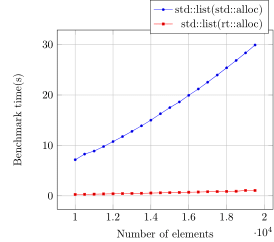
\includegraphics[scale=0.5]{fig/std_list_bench.png} }
%    \subfloat[]{ 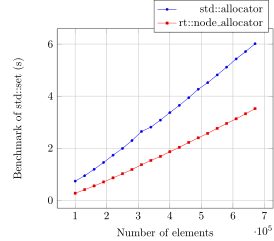
\includegraphics[scale=0.5]{fig/std_set_bench.png} }
%        \\
%    \caption[Benchmarks]
%    {Never slower than blah.}
%    \label{fig::bench}
%\end{figure}


\section{Impact on the Standard} \label{impact}

The Following additions are required in the standard.

\subsection{New \texttt{std::allocator\_traits} members}

We require the addition of two new member function and
a typedef in \texttt{std::allocator\_traits()} as follows

\medskip
\begin{lstlisting}
template<class Alloc>
struct allocator_traits {
  // Equal to Alloc::node_allocation_only if present,
  // std::false_type otherwise. Array allocation with
  // allocate(n) is ruled out if it is std::true_type.
  using node_allocation_only = std::false_type

  // Calls a.allocate_node() if present otherwise calls
  // Alloc::allocate(1). Memory allocate with this function
  // must be deallocated with deallocate_node.
  pointer allocate_node(Alloc& a);

  // Calls a.deallocate_node(pointer) if present otherwise
  // calls Alloc::deallocate(p, 1). Can only be used with
  // memory allocated with allocate_node.
  void deallocate_node(Alloc& a, pointer p);
};
\end{lstlisting}
%The behaviour of these new members is better explained in section \ref{impact}.
These additions provide the following options inside node-based
containers
\begin{enumerate}
\item {\bf Array allocation only}.
This is the {\it status quo}. Libraries can continue to call
\texttt{allocate(n)} if they want, but since the majority of implementations
use $n = 1$, they may simply be implemented in terms of
\texttt{allocate\_node()}, regardless of whether the allocator provides this
function or not. The implementation of \texttt{allocate\_node()} in
\texttt{std::allocator\_traits} should fall back to \texttt{allocate(1)} 
when the allocator does not provide one.

\item {\bf Node allocation only}.
In this case, the user is required to set the typedef \texttt{node\_allocation\_only}
to \texttt{std::true\_type} in the allocator and provide \texttt{allocate\_node()}. The user is
not required to provide \texttt{allocate(n)}.
\item {\bf Array and node allocation together}. It is possible to use
both array {and} node allocation when the user provides \texttt{allocate\_node}
and sets \texttt{node\_allocation\_only} to \texttt{std::false\_type}.
I am unaware if this option is useful.
\end{enumerate}

\subsection{The node type}

We require the following node iterface on node based containers

\medskip
\begin{lstlisting}
template <class T, class Ptr>
struct node_type {
  using value_type = T;
  using pointer = // Usually taken from std::pointer_traits<Ptr>
  template<class U, class K>
  struct rebind { using other = node_type<U , K>; };
};
\end{lstlisting}

We also require the node type to be independent of the container
and of the compare type. The following code should compile.

\medskip
\begin{lstlisting}
  using set_type1 = rt::set<T, C1, A1>;
  using set_type2 = rt::set<T, C2, A2>;

  using pointer = // Arbitray pointer type.
  using node_type1 =
    typename set_type1::node_type::template rebind<T, pointer>;
  using node_type2 = typename
    set_type2::node_type::template rebind<T, pointer>;
  static_assert(std::is_same<node_type1, node_type2>::value,"");
\end{lstlisting}

The following containers are affected: \texttt{std::forward\_list},
\texttt{std::list}, \texttt{std::set}, \texttt{std::multiset},
\texttt{std::unordered\_set}, \texttt{std::unordered\_multiset},
\texttt{std::map}, \texttt{std::multimap},
\texttt{std::unordered\_map}, \texttt{std::unordered\_multimap}

\section{Acknowledgment}

I would like thank people that gave me any kind of feedback: Ville Voutilainen,
Nevin Liber, Daniel Gutson, Alisdair Meredith, David Krauss. Special thanks go
to Ion Gaztañaga for suggesting important changes in the original design.

\begin{thebibliography}{9}

  \bibitem{middleditch} Sean Middleditch, \url{http://www.open-std.org/jtc1/sc22/wg21/docs/papers/2015/p0038r0.html}
  \bibitem{chandler} Chandler Carruth, {\it Efficiency with Algorithms, Performance
  with Data Structures} (\url{https://www.youtube.com/watch?v=fHNmRkzxHWs})
  \bibitem{meyers} Scott Meyers, {\it Cpu Caches and Why You Care} (\url{https://www.youtube.com/watch?v=WDIkqP4JbkE})
  \bibitem{boost} \url{http://www.boost.org/doc/libs/1_58_0/boost/container/node_allocator.hpp}
  \bibitem{prop1} Ion Gazta\~ naga, \url{http://www.open-std.org/jtc1/sc22/wg21/docs/papers/2006/n2045.html}
  \bibitem{rtcpp} \url{https://github.com/mzimbres/rtcpp}
  \bibitem{alexandrescu} Andrei Alexandrescu, {\it std::allocator Is to Allocation what
  std::vector Is to Vexation} (\url{https://www.youtube.com/watch?v=LIb3L4vKZ7U})
  \bibitem{embedded} \url{http://www.open-std.org/pipermail/embedded/2014-December/000335.html}
  \bibitem{proplist} \url{https://groups.google.com/a/isocpp.org/forum/#!topic/std-proposals/ccwOpTxM_xE}
  \bibitem{scary} \url{http://www.open-std.org/jtc1/sc22/wg21/docs/papers/2009/n2980.pdf}

\end{thebibliography}

\appendix

\section{Alternative approaches} \label{alternative}

There are other possible approaches to support node allocation that are worth knowing
of.  I will list them here, so that the commitee can compare them.

\subsection{\texttt{allocate(n)} with $n = 1$}

%\medskip
%\noindent
%{\bf Ensure \texttt{allocate(n)} is called with $n = 1$}.
This seems the easiest
way to perform node allocation. Once the standard guarantees $n$ will be always $1$,
there is no more need to provide array allocation for node-based containers. The
parameter $n$ can be simply ignored. The \texttt{allocate} and \texttt{deallocate}
can be implemented in terms of node-allocation-only functions, for example
\medskip
\begin{lstlisting}
pointer allocate(std::size_t /* n is ignored */)
{
  return allocate_node();
}

void deallocate(pointer p, std::size_t /* n is ignored */)
{
  deallocate_node();
}
\end{lstlisting}

The problem with this approach is that it prevents array allocation inside
node-based containers, which means it can be viewed as a narrowing of the
current interface.

\subsection{Provide a \texttt{constexpr max\_size()} that returns 1}

%\medskip
%\noindent
%{\bf Provide a \texttt{constexpr max\_size()} that returns 1}.

This scheme
can achieve the same goals as my main proposal and does not require any
addition to \texttt{std::allocator\_traits}. Libraries should check if
\texttt{max\_size()} can be evaluated at compile time and take appropriate
action i.e. ensure \texttt{allocate(n)} is always called with $n = 1$.
I did not adopted it due to some disadvantages I see with it

\begin{enumerate}
\item It does not make containers implementation simpler.

\item Function names should reflect that array and node allocation have
different semantics, apart from the storage size. If memory expansion (realloc)
is added in the future, it should only work with storage allocated with
\texttt{allocate(n)} but not with storage allocated for nodes. This allows node
allocations to avoid extra bookeeping data to mark the storage as
non-expandable.

\item It requires the user to specialize \texttt{std::allocator\_traits} to
provide a \texttt{constexpr max\_size()} since the default is not
\texttt{constexpr}. This is not bad but I prefer to avoid it if I can.

\item Other static information like \texttt{propagate\_on\_container\_copy\_assignment}, etc,
are provided as typedef so I prefer to keep the harmony.

\item It sounds more like a hack of the current allocator interface to achieve
node allocation than a full supported feature.

\end{enumerate}

\newpage

\section{Node type and safer allocator} \label{saferalloc}

\medskip
\begin{lstlisting}
  // Buffer where nodes are allocated.
  std::array<char, 1000> buffer = {{}};

  // SCARY aware node type. It does not matter from which
  // allocator it was taken since we can rebind it.
  using node_type = rt::set<int>::node_type;

  // The user node allocator type and its instance.
  using alloc_type = rt::node_allocator<int, node_type>;
  alloc_type alloc(buffer);

  // Ok, Perform array allocation on int's
  auto a = alloc.allocate(10);

  // Error, node allocation only for node_type
  auto a = alloc.allocate_node(); // Compile time error

  // The folowing lines occurs inside the unordered container.
  // Rebinds to the unordered container internal node_type2.
  // It is equal to node_type except that it may have a
  // different pointer type.
  using node_alloc_type =
    typename alloc_type::template rebind<node_type2>::other;

  node_alloc_type node_alloc(alloc);

  // Error, array allocation disable for node_type.
  auto b = node_alloc.allocate(10); // Error

  // Ok, Perform node allocation on the node type
  auto b = node_alloc.allocate_node(); // Ok

  // Rebinds to the unordered container internal array
  // allocation type, let us say it is double* (just an example). 
  using array_alloc_type =
    typename alloc_type::template rebind<double*>::other;
  array_alloc_type array_alloc(alloc);

  // Ok, array allocation enable. This is not the node type.
  auto c = alloc.allocate(10); // Ok

  // Error, node alocation is not enabled for double*.
  auto c = alloc.allocate_node(); // Error
\end{lstlisting}

\end{document}

